\documentclass[11pt,a4j,notitlepage]{jreport}

\usepackage{times}
\usepackage[dvipdfmx]{graphicx}	%図を表示するのに必要
\usepackage[dvipdfmx]{color}	%jpgなどを表示するのに必要
\usepackage{amsmath,amssymb}	%数学記号を出すのに必要
\usepackage{setspace}
\usepackage{bm}
\usepackage{braket}	%ブラケットを表示するのに必要
\usepackage{otf}
\usepackage{here}	%図を好きな位置に表示
\usepackage[subrefformat=parens]{subcaption}	%サブキャプション

%PDFの機能(しおり機能、ハイパーリンク機能)が使えるようにする
%しおりの文字化けを防ぐ
\usepackage{atbegshi}
\AtBeginShipoutFirst{\special{pdf:tounicode 90ms-RKSJ-UCS2}}
%hyperrefのverが2007-06-14 6.76i以前の時は↓
%\AtBeginShipoutFirst{\special{pdf:tounicode 90ms-RKSJ-UCS2}}
\usepackage[dvipdfmx,bookmarkstype=toc,colorlinks=true,urlcolor=blue,linkcolor=blue,
citecolor=blue,linktocpage=true,bookmarks=true,setpagesize=false,
pdftitle={量子状態トモグラフィー},
pdfauthor={小林哲也},%
pdfsubject={Bachelor's thesis in 2020}]{hyperref}
\usepackage[numbers,sort]{natbib}
\usepackage{tocbibind}%目次、表一覧、図一覧をしおりに入れる
 
%式、図、表番号の付け方の再定義
\makeatletter
	\renewcommand{\theequation}{%
	\thesection.\arabic{equation}}
	\@addtoreset{equation}{section}
	\def\thefigure{\thesection.\arabic{figure}}
	\@addtoreset{figure}{section}
	\renewcommand{\thetable}{%
	\thesection.\arabic{table}}
	\@addtoreset{table}{section}
\makeatother

%本文と図の余白
\setlength\intextsep{30pt} 
 
\renewcommand\bibname{参考文献}	%関連図書の表示を参考文献に変更
\newcommand{\fig}[1]{図~\ref{#1}}	%図の引用の再定義
\newcommand{\tab}[1]{表~\ref{#1}}	%表の引用の再定義
\newcommand{\eq}[1]{式~\eqref{#1}}	%式の引用の再定義
 
%大きなフォントの定義(表紙用)
\def\HUGE{\fontsize{32pt}{36pt}\selectfont} %\fontsize{フォントの大きさ}{baselineskip}
 
 
%本文
\begin{document}

	%タイトル
	\begin{titlepage}
		\begin{center}\begin{LARGE}
			\vspace{1em}
			{令和元年度}\\
			\vspace{1.5em}
			{卒業研究}\vspace{3em}\\
			\textbf{\HUGE 量子状態トモグラフィー}\\
			\vspace{4em}
			{\LARGE 指導教員}\\
			\vspace{0.8em}
			{\Huge\bf 山本 俊 教授}\\
			\vspace{0.2\vsize}
			{大阪大学 基礎工学部\\ 電子物理科学科 物性物理科学コース\\ 山本研究室\\学籍番号 09D16031}\\
			\vspace{0.8em}
			{\Huge\bf 小林哲也}\\
			\vspace{3em}
			{\Large 2020年3月6日}
		\end{LARGE}\end{center}
	\end{titlepage}

	%目次のページだけローマ数字に設定
	\pagenumbering{roman}

	%目次サブセクションまで表記
	\setcounter{tocdepth}{2}
	\tableofcontents

	\clearpage

	%図目次
	\listoffigures

	%ページ数をリセットしアラビア数字に変更
	\clearpage
	\pagenumbering{arabic}


	\chapter{序論}
	\section{研究の背景と目的}

	近年注目を増している量子情報、量子コンピューティング研究・開発において実験的に生成された量子状態を正確に認識することは極めて重要である。
	しかし、任意の量子状態を特定するには有限回の測定では不可能であり、実験的に真の量子状態を知ることは困難である。
	そこで、量子状態トモグラフィーが用いられる。
	量子状態トモグラフィーとは、同じ量子状態を複数生成し、それぞれを測定基底を変えて測定をすることで得られた観測データから、最尤推定などを用いて真の量子状態を推定することである。
	本論文では、量子状態トモグラフィーの一般的理論を説明した後、実験的誤りに対する耐性があるアルゴリズムを紹介する。
	最後に、これらのアルゴリズムを疑似実験データを利用して、4 qubitsや2 qutritsの場合についてPythonで実装する。


	\chapter{理論}
	\section{量子状態トモグラフィーの一般的理論}


	\subsection{密度行列}

	量子状態は密度行列によって表される。密度行列$\hat{\rho}$とは以下二つの性質を満たす正方行列である。
	\begin{equation}
		Tr[\hat{\rho}]=1
		\label{eq2.1}
	\end{equation}
	また、密度行列の固有値を$\lambda$とすると、
	\begin{equation}
		0 \leq \lambda \leq 1, \ \ \ \  ^\forall \lambda
		\label{eq2.2}
	\end{equation}
	本論文では$d$次元の密度行列を$\hat{\rho}_d$と表記する。



	\subsection{1 qubitトモグラフィー (直交基底測定)}

	qubitは$2$次元の密度行列で表される。

	1 qubitトモグラフィーのために、パウリ演算子を導入する。パウリ演算子は単位演算子$I$と$SU(2)$の$X,\ Y,\ Z$からなる。
	\begin{equation}
		\begin{aligned}
			I \equiv \hat{\lambda}_0 = \begin{pmatrix} 1 & 0 \\ 0 & 1 \end{pmatrix}&,\ \ X \equiv \hat{\lambda}_1 = \begin{pmatrix} 0 & 1 \\ 1 & 0 \end{pmatrix}\\
			Y \equiv \hat{\lambda}_2 = \begin{pmatrix} 0 & -i \\ i & 0 \end{pmatrix}&,\ \ Z \equiv \hat{\lambda}_3 = \begin{pmatrix} 1 & 0 \\ 0 & -1 \end{pmatrix}
		\end{aligned}
		\label{eq2.3}
	\end{equation}
	これらを用いて、1 qubitの密度行列$\hat{\rho}_2$は次のように表される。
	\begin{equation}
		\hat{\rho}_2 = \frac{1}{2} \sum_{j=0}^3 r_j \hat{\lambda}_j, \ \ \ \ r_j \in Re
		\label{eq2.4}
	\end{equation}
	$SU(2)$はトレースが0なので、密度行列$\hat{\rho}_2$は規格化のために$r_0 = 1$を満たす必要がある。また、ほかのパラメータ$r_{j=1,...,3}$は
	\begin{equation}
		r_1^2 + r_2^2 + r_3^2 \leq 1
		\label{eq2.5}
	\end{equation}
	のみ満たす。また、$r_j$は$r_j = Tr[\hat{\rho}_2 \hat{\lambda}_j]$で得られる。\\
	
	したがって、1 qubitの密度行列は
	\begin{equation}
		\hat{\rho}_2 = \frac{1}{2} \begin{pmatrix}
			1 + \braket{\hat{\lambda}_3} &
			\braket{\hat{\lambda}_1} - i \braket{\hat{\lambda}_2} \\
			\braket{\hat{\lambda}_1} + i \braket{\hat{\lambda}_2} &
			1 - \braket{\hat{\lambda}_3}
			\end{pmatrix}
	\end{equation}
	で表される。
	
	上式から、1 qubitの密度行列は3つの測定だけで求まりそうだが、実験的には4つ目の基底$\hat{\lambda}_0$の測定によって密度行列の規格化が必要である。また、$\langle \hat{\lambda}_j \rangle$の値によっては、$(2.1.2)$式を満たさないことがある。したがって、最尤推定などを用いて物理的に意味のある密度行列を見つける必要がある。

	$SU(2)$生成子は必ず物理的状態を示すとは限らないが、$\hat{\lambda}_{0,...,3}$は常に物理的に意味のある状態の密度行列の線形和で表すことができる。例えば、パウリ演算子は光学系での測定としては物理的意味がない。しかし、光子の測定を偏向基底で行う際に以下のようなものが用いられる。
	\begin{equation}
		\begin{aligned}
			\ket{H} \bra{H} = \frac{1}{2}[\hat{\lambda}_0 + \hat{\lambda}_3] \ket{V} \bra{V} = \frac{1}{2}[\hat{\lambda}_0 - \hat{\lambda}_3]\\
			\ket{D} \bra{D} = \frac{1}{2}[\hat{\lambda}_0 + \hat{\lambda}_1] \ket{L} \bra{L} = \frac{1}{2}[\hat{\lambda}_0 + \hat{\lambda}_2]
		\end{aligned}
	\end{equation}
	ここで、$\ket{H} = \ket{0}, \ \ket{V} = \ket{1}, \ \ket{D} = (\ket{0} + \ket{1}) / \sqrt{2} , \ \ket{L} = (\ket{0} + i\ket{1}) / \sqrt{2}$

	このようにどの直交した測定基底を選んでも他のいくつかの測定演算子$\hat{\Pi}_k$を用いて$\hat{\lambda}_j = \frac{1}{2} \sum_{k} a_{jk} \hat{\Pi}_k$と表すことができる。そして、トモグラフィーは測定結果$a_{jk} = \langle \hat{\Pi}_k \rangle = Tr[\hat{\rho}_2 \hat{\Pi}_k]$を測定することで行われる。

	\subsection{1 qubitトモグラフィー (非直交基底測定)}

	実際には、測定は測定装置側の基底を偏向せずに量子状態を変化させて測定する。そのため、1 qubitの状態を測定基底に合わせて、$| 0 \rangle + | 1 \rangle$や$| 0 \rangle + i | 1 \rangle$から$| 0 \rangle$へ量子状態を変化させることが難しい場合がある。その場合、測定基底を$| 0 \rangle$と
	\begin{equation}
		\begin{aligned}
			\ket{\theta_+} &= \frac{1}{\sqrt{2}} [\cos \theta \ket{0} + \sin \theta \ket{1}]\\
			\ket{\varphi_+} &= \frac{1}{\sqrt{2}} [\cos \varphi \ket{0} + i \sin \varphi \ket{1}]
		\end{aligned}
	\end{equation}
	とすることができる。$\theta, \varphi$は小さい値でもよい。つまり、1 qubitトモグラフィーはある測定基底と少しの摂動があれば行える。実験系によってはこれは重要になることがある。

	任意の基底$\ket{\psi_\nu}$での測定は射影子$\hat{\lambda}_\nu = \ket{\psi_\nu} \bra{\psi_\nu}$で表され、これらの基底による観測回数$n_\nu$は
	\begin{equation}
		n_\nu = \mathcal{N} \braket{\psi_\nu | \hat{\rho} | \psi_\nu}
	\end{equation}
	で表される。($\mathcal{N}$は定数)

	\subsection{Quditへの拡張}

	まず、$SU(d)$を準備する。($d$次元の$SU$群)

	$d$次元の要素行列$\{ e_j^k|k,j=1,...,d \}$は
	\begin{equation}
		\big( e_j^k \big) _{\mu \nu} = \delta_{\nu j} \delta_{\mu k}, \ \ \ \ 1 \leq \nu, \mu \leq d
	\end{equation}
	で表され、$\mu$行$\nu$列目の要素が1で他の要素すべてが0である行列である。

	これらの行列は交換関係を満たす。
	\begin{equation}
		\big[ e_j^i, e_l^k \big] = \delta_{kj} e_l^i - \delta_{il} e_j^k
	\end{equation}
	$d(d-1)$個のトレースが0の行列が存在する。
	\begin{equation}
		\begin{aligned}
			\Theta_j^k = e_j^k + e_k^j, \ \ \beta_j^k = -i \big( e_j^k - e_k^j \big) \ \ \ \ \ \ \ \ 1 \leq k < j \leq d
		\end{aligned}
	\end{equation}
	これらは$SU(d)$群の非対角生成子である。

	対角生成子として残り$d-1$個のトレースが0の行列を
	\begin{equation}
		\eta_r^r = \sqrt{\frac{2}{r(r-1)}} \Biggl[ \sum_{j=1}^r e_j^j - r e_{r+1}^{r+1} \Biggr]
	\end{equation}
	とすると、これで$d^2-1$個の生成子が得られる。\\
	ここで$\lambda$行列を次のように定義する。
	\begin{equation}
		\begin{aligned}
			\hat{\lambda}_{(j-1)^2 + 2(k-1)} &= \Theta_j^k\\
			\hat{\lambda}_{(j-1)^2 + 2k-1} &= \beta_j^k\\
			\hat{\lambda}_{j^2-1} &= \eta_{j-1}^{k-1}
		\end{aligned}
	\end{equation}
	$d$次元に拡張してもこれらの形式は完全エルミート演算子基底である。つまり、$\hat{\lambda}$がエルミートかつ次式を満たす。
	\begin{equation}
		\sum_{j=0}^{d^2 - 1} \hat{\lambda}_j = \hat{1}
	\end{equation}

	$d$次元に拡張しても$(2.1.4)$式はそのまま適用できる。つまり、密度行列$\hat{\rho}_d$は生成子の線形結合で表される。
	\begin{equation}
		\hat{\rho}_d = \frac{1}{d} \sum_{j=0}^{d^2 - 1} r_j \hat{\lambda}_j
	\end{equation}
	これは1 quditの密度行列である。規格化のために係数$r_0$は1とし、$Tr \big[ \hat{\rho}_d^2 \big] \leq 1$より$\sum_{j=1}^{d^2 - 1} r_j^2 \leq d(d-1)/2$を満たす。

	\subsection{Multi quditsへの拡張}

	Multi qubitsでは、演算子のヒルベルト空間を規格化された単位行列$\hat{\lambda}_0$を含んだ$SU(2)$を生成子のテンソル積で定義する。
	\begin{equation}
		SU(2) \otimes SU(2) \otimes ・・・ \otimes SU(2)
	\end{equation}

	2 quditsでは$d^2$の次元を持った密度行列$\hat{\rho}_{2 d}$は同様に拡張できる。\\
	$\hat{\lambda}_0$を含む$\hat{\lambda}$行列のテンソル積$\hat{\lambda}_{j 1} \otimes \hat{\lambda}_{j 2}$のすべての組はそれぞれ線形独立なので、$\hat{\rho}_{2 d}$は次のように表される。
	\begin{equation}
		\hat{\rho}_{2 d} = \frac{1}{d^2} \sum_{j1,j2=0}^{d^2 - 1} r_{j 1, j 2} \hat{\lambda}_{j 1} \otimes \hat{\lambda}_{j 2}
	\end{equation}
	同様に、n quditsでは
	\begin{equation}
		\hat{\rho}_{n d} = \frac{1}{d^n} \sum_{j1,...,jn=0}^{d^2 - 1} r_{j 1,...,j n} \hat{\lambda}_{j 1} \otimes ・・・ \otimes \hat{\lambda}_{j n}
	\end{equation}

	\subsection{密度行列の再構成}

	簡単のために$\hat{\Gamma}_\nu = \hat{\lambda}_{j 1} \otimes ・・・ \otimes \hat{\lambda}_{j n}$とすると、密度行列は
	\begin{equation}
		\hat{\rho}_{n d} = \sum_{\nu = 0}^{d^n - 1} \tilde{r}_\nu \hat{\Gamma}_\nu
	\end{equation}
	で表される。$\tilde{r}_\nu$は$d^n$要素あるベクトルの$\nu$番目の要素で
	\begin{equation}
		\tilde{r}_\nu = Tr \big[ \hat{\Gamma}_\nu \hat{\rho}_{n d} \big]
	\end{equation}
	これを$(2.1.9)$式に代入して
	\begin{equation}
		n_\nu = \mathcal{N} \sum_{\mu = 0}^{d^n - 1} B_{\nu, \mu} \tilde{r}_\nu
	\end{equation}
	ここで、$B_{\nu, \mu}$は$d^n \times d^n$行列の$\nu$行$\mu$列番目の要素で
	\begin{equation}
		B_{\nu, \mu} = \braket{\psi_\nu | \hat{\Gamma}_\mu | \psi_\nu}
	\end{equation}
	$B_{\nu, \mu}$が可逆行列であれば
	\begin{equation}
		\tilde{r}_\nu = \mathcal{N}^{-1} \sum_{\nu = 0}^{d^n - 1} \hat{M}_\nu n_\nu = \sum_{\nu = 0}^{d^n - 1} \hat{M}_\nu s_\nu
	\end{equation}
	ここで、$\hat{M}_\nu$は$d \times d$行列で
	\begin{equation}
		\hat{M}_\nu = \sum_{\nu = 0}^{d^n - 1} \big( B^{-1} \big)_{\nu, \mu} \hat{\Gamma}_\nu
	\end{equation}
	$\hat{M}_\nu$の性質から
	\begin{equation}
		\sum_\nu Tr \big[ \hat{M}_\nu \big] \ket{\psi_\nu} \bra{\psi_\nu} \hat{\rho}_{n d} = \hat{\rho}_{n d}
	\end{equation}
	両辺でトレースをとると
	\begin{equation}
		\sum_\nu Tr \big[ \hat{M}_\nu \big] n_\nu = \mathcal{N}
	\end{equation}
	したがって、任意の密度行列$\hat{\rho}_{n d}$は次のように再構成される。
	\begin{equation}
		\hat{\rho}_{n d} = \frac{\sum_\nu \hat{M}_\nu n_\nu}{\sum_\nu Tr \big[ \hat{M}_\nu \big] n_\nu} 
	\end{equation}


	\section{最尤推定}

	これで密度行列は実験の測定基底と観測回数によって一意に求まるが、これまでで求まる密度行列は必ずしも密度行列の性質をすべて満たしているとは限らない。

	この問題を避けるために最尤推定を利用する。手順は以下の通りである。

	\begin{enumerate}
		\item \underline{密度行列の性質を満たす密度行列を生成する}
		\item \underline{1で求めた密度行列が非物理的であれば尤度関数を導入し、次の最尤推定を行う}
		\item \underline{Iterativeなアルゴリズムを用いて尤度関数を最大化させもっとも確からしい密度行列を求める}
	\end{enumerate}


	\subsection{密度行列の確認}

	まず、密度行列の性質を満たす行列を生成する。

	半正定値行列$\hat{G}$は次の式を満たすとする。
	\begin{equation}
		\braket{\psi | \hat{G} | \psi} \geq 0,\ \ \ \ \ ^\forall \ket{\psi}
	\end{equation}
	$\hat{G} = \hat{T}^\dagger \hat{T}$と書けるどんな行列$\hat{G}$も必ず半正定値行列となる。実際、
	\begin{equation}
		\braket{\psi | \hat{T}^\dagger \hat{T} | \psi} = \braket{\psi' | \psi'} \geq 0
	\end{equation}
	ここで、$\ket{\psi'} = \hat{T} \ket{\psi}$である。さらに、$(\hat{T}^\dagger \hat{T})^\dagger = \hat{T}^\dagger (\hat{T}^\dagger)^\dagger = \hat{T}^\dagger \hat{T}$、すなわち$\hat{G}$はエルミートである。

	規格化のために
	\begin{equation}
		\hat{g} = \frac{\hat{T}^\dagger \hat{T}}{Tr \big[ \hat{T}^\dagger \hat{T} \big] } 
	\end{equation}
	とすると、$\hat{g}$は密度行列の数学的条件をすべて満たす。

	この性質を利用するために、$\hat{T}$を$d^2$個の実数変数$t$を用いて、
	\begin{equation}
		\hat{T}_{(t)} = \begin{pmatrix}
			t_1 & 0 & & \cdots & 0 \\
			t_{d+1} + it_{d+2} & t_2 & & & \\
			\vdots & & \ddots &  & \vdots \\
			& & & t_{d-1} & 0 \\
			t_{d^2 - d + 1} + it_{d^2 - d + 2} & & \cdots & t_{d^2 - 1} + it_{d^2} & t_d
		\end{pmatrix}
	\end{equation}
	とすると、
	\begin{equation}
		\hat{\rho}_p = \frac{\hat{T}^\dagger_{(t)} \hat{T}_{(t)}}{Tr \big[ \hat{T}^\dagger_{(t)} \hat{T}_{(t)} \big] }
	\end{equation}
	は明らかに密度行列の性質を持つ。
	つまり、この複素行列$\hat{T}_{(t)}$を実験値から適切に求めることで最も確からしい密度行列が求められる。

	そこで、$(2.1.28)$式で実験値から求めた密度行列が$(2.2.5)$式となっているかを確認する。
	$(2.2.5)$式は複素数のCholesky分解そのものであるので、確認するのは容易である。[\autoref{chap:Cholesky}]
	ここで求めた複素行列$\hat{T}_{(t)}$が上述の条件を満たしていれば、以降の最尤推定は必要ない。

	最尤推定が必要な場合、得られた密度行列は非物理的な値になっているので、最尤推定の初期値としてそのまま利用することはできない。
	実験的なデータ誤差や偏りに左右されないように最大混合状態$\hat{I}$を最尤推定の初期値とすることは合理的である。
	しかし、今回は真の密度行列をある程度推測してから最尤推定を行うことで計算時間を短縮できる仮定のもとに、初期値を実験データを利用して求めた密度行列にする場合も考える。
	つまり、$(2.2.4)$式の制約から対角項を実数のみ利用し求めた密度行列を初期値とする。
	また、計算途中で0の除算が発生した場合は0の代わりに微小項を代入する。

	\subsection{$\hat{R}\hat{\rho}\hat{R}アルゴリズム$}

	まず、尤度関数$\mathcal{L} (\hat{\rho})$を導入する。

	一般の測定$\hat{\Pi}$はPOVMで表されるので、$Tr \big[ \hat{\Pi}_i \hat{\rho} \big] \geq 0$を満たす。
	ここで、総測定回数を$N$、それぞれの測定基底$\hat{\Pi}_i$における測定回数を$f_i$とする。
	量子状態$\hat{\rho}$におけるある測定回数の集合{$f_i$}の尤度関数は$\mathcal{L} (\hat{\rho}) = \prod_i \Pr_i^{f_i}$で得られる。
	$\Pr_i = Tr \big[ \hat{\Pi}_i \hat{\rho} \big]$はそれぞれの基底で得られる確率である。
	最終的な目標はこの尤度関数を最大化させる密度行列$\hat{\rho}_0$を見つけることである。
	ここで相対頻度を$\tilde{f}_i = \frac{f_i}{N}$とする。
	$\ket{y_i}$は正規直交基底として、測定基底を$\hat{\Pi}_i = \ket{y_i} \bra{y_i}$とする。
	また、POVMは完全関係を満たすので、
	\begin{equation}
		\sum_i \ket{y_i} \bra{y_i} = \hat{I}
	\end{equation}

	\subsection*{\underline{尤度関数の増加}}

	対数尤度関数は$\log \mathcal{L} (\hat{\rho}) = \sum_i \tilde{f}_i \log \Pr_i$である。ここで、
	\begin{equation}
		\hat{R} = \sum_i \frac{\tilde{f}_i}{\Pr_i} \ket{y_i} \bra{y_i}
	\end{equation}
	とすると、$\hat{R} \hat{\rho}$の対数尤度関数は
	\begin{equation}
		\begin{aligned}
			\log \mathcal{L} \big( \hat{R} \hat{\rho}) &= \sum_i \tilde{f}_i \log \Big( Tr \big[ \hat{\Pi}_i \hat{R} \hat{\rho} \big] \Big) \\
			&=  \sum_i \tilde{f}_i \log \Bigg( Tr \Big[ \hat{\Pi}_i \sum_j \frac{\tilde{f}_j}{\Pr_j} \ket{y_j} \bra{y_j} \hat{\rho} \Big] \Big) \\
			&= \sum_i \tilde{f}_i \log \Bigg( \sum_j \frac{\tilde{f}_j}{\Pr_j} \braket{y_i | y_j} \braket{y_j | \hat{\rho} | y_i} \Bigg) \\
			&= \sum_i \tilde{f}_i \log \tilde{f}_i
		\end{aligned}
	\end{equation}
	となる。したがって、$\hat{R}$による密度行列の更新前後の対数尤度関数の差は
	\begin{equation}
		\log \mathcal{L} \big( \hat{R} \hat{\rho} \big) - \log \mathcal{L} \big( \hat{\rho} \big) = \sum_i \tilde{f}_i \log \tilde{f}_i - \sum_i \tilde{f}_i \log \Pr_i = \sum_i \tilde{f}_i \log \frac{\tilde{f}_i}{\Pr_i}
	\end{equation}
	ここで、$\sum_i \tilde{f}_i = \sum_i \Pr_i = 1,\ \ 0 < \tilde{f},\ \ \Pr_i < 1$なので、Jensenの不等式
	\begin{equation}
		\prod_i \Big[ \frac{x_i}{a_i} \Big]^{\tilde{f}_i} \leq \sum_i \tilde{f}_i \frac{x_i}{a_i} \ \ \ \ \Big( \sum_i x_i = 1,\ x_i \geq 0,\ a_i > 0 \Big)
	\end{equation}
	を用いると、
	\begin{equation}
		\begin{aligned}
			- \sum_i \tilde{f}_i \log \frac{\tilde{f}_i}{\Pr_i} &= \sum_i \tilde{f}_i \log \frac{\Pr_i}{\tilde{f}_i} \\
			&= \log \Bigg( \prod_i \Big( \frac{\Pr_i}{\tilde{f}_i} \Big)^{\tilde{f}_i} \Bigg) \\
			&\leq \log \Big( \sum_i \tilde{f}_i \frac{\Pr_i}{\tilde{f}_i} \Big) \\
			&= \log 1 = 0
		\end{aligned}
	\end{equation}
	したがって、$\hat{\rho}^{(k+1)} = \hat{R} (\hat{\rho}^{(k)}) \hat{\rho}^{(k)}$と密度行列を更新していけば尤度関数は必ず増加する。

	\subsection*{\underline{尤度関数の収束性}}

	Jensenの不等式から
	\begin{equation}
		\prod_i \Big[ \frac{x_i}{a_i} \Big]^{\tilde{f}_i} \leq \sum_i \tilde{f}_i \frac{x_i}{a_i} \Longleftrightarrow \prod_i x_i^{\tilde{f}_i} \leq \prod_i a_i^{\tilde{f}_i} \sum_k \tilde{f}_k \frac{x_k}{a_k}
	\end{equation}
	より、尤度関数は
	\begin{equation}
		\begin{aligned}
			\mathcal{L} (\hat{\rho}) &= \prod_i Tr \big[ \ket{y_i} \bra{y_i} \hat{\rho} \big]^{\tilde{f}_i} \\
			&\leq \prod_i a_i^{\tilde{f}_i} \sum_k \tilde{f}_k \frac{Tr [ \ket{y_i} \bra{y_i} \hat{\rho}]}{a_k} \\
			&= \prod_i a_i^{\tilde{f}_i} Tr \big[ \hat{\rho} \hat{R} (a) \big]
		\end{aligned}
	\end{equation}
	\begin{equation}
		\hat{R} (a) = \sum_i \frac{\tilde{f}_i}{a_i} \ket{y_i} \bra{y_i}
	\end{equation}
	ここで、任意の半正定値演算子$\hat{R} = \sum_i \lambda_i \ket{y_i} \bra{y_i},\ \lambda_i \geq 0$の最大固有値を$\max_i \lambda_i$とすると、
	\begin{equation}
		Tr [\hat{\rho} \hat{R}] \leq \max_i \lambda_i
	\end{equation}
	よって、$\hat{R} (a)$の最大固有値を$\lambda (y, a)$として、
	\begin{equation}
		\mathcal{L} (\hat{\rho}) \leq \lambda (y, a) \prod_i a_i^{\tilde{f}_i}
	\end{equation}
	最大固有ベクトルを$\ket{\psi(y, a)}$とすると、等式が成立するのは
	\begin{equation}
		\frac{| \braket{y_i | \psi (y, a)} |^2}{a_i} = const
	\end{equation}
	これにより、尤度関数の上限が存在することがわかる。\\

	これまでで、$\hat{\rho}^{(k+1)} = \hat{R} (\hat{\rho}^{(k)}) \hat{\rho}^{(k)}$は$\hat{R}$が対角行列または$\hat{\rho}$が対角行列であれば最尤推定が可能であることが示された。
	しかし、密度行列は非対角項も考慮する必要があり、実験による測定もPOVMとは限らない。
	そこで、密度行列の収束性を利用して$\hat{R} (\hat{\rho}_0) \hat{\rho}_0 \hat{R} (\hat{\rho}_0) = \hat{\rho}_0$となる$\hat{\rho}_0$が存在すると仮定して、規格化定数$\mathcal{N}$を用いて
	\begin{equation}
		\hat{\rho}^{(k+1)} = \mathcal{N} \big[ \hat{R} (\hat{\rho}^{(k)}) \hat{\rho}^{(k)} \hat{R} (\hat{\rho}^{(k)}) \big]
	\end{equation}
	を$\hat{R} \hat{\rho} \hat{R}$アルゴリズムと呼ぶことにする。

	一般に、$\hat{R} \hat{\rho} \hat{R}$アルゴリズムは尤度関数が常に増加するとは言えない。
	そこで、非負の値$\epsilon$を導入することでこの問題を解決する。

	\subsection{Diluted $\hat{R} \hat{\rho} \hat{R}$アルゴリズム}

	Diluted $\hat{R} \hat{\rho} \hat{R}$アルゴリズムとは以下の式で表す。
	\begin{equation}
		\hat{\rho}^{(k+1)} = \mathcal{N} \Bigg[ \frac{\hat{I} + \epsilon \hat{R} (\hat{\rho}^{(k)})}{1+\epsilon} \hat{\rho}^{(k)} \frac{\hat{I} + \epsilon \hat{R} (\hat{\rho}^{(k)})}{1+\epsilon} \Bigg]
	\end{equation}
	$\epsilon \ll 1$であれば尤度関数は常に増加する。

	\subsection*{\underline{尤度関数の増加}}

	$\epsilon \ll 1$で$(2.2.19)$式の$\epsilon$の1次までの近似をとると、$(1 + \epsilon)^{-2} \approx 1 - 2\epsilon$より、
	\begin{equation}
		\hat{\rho}^{(k+1)} = \hat{\rho}^{(k)} + \Delta \hat{\rho}
	\end{equation}
	\begin{equation}
		\Delta \hat{\rho} = \epsilon \big( \hat{R} \hat{\rho}^{(k)} + \hat{\rho}^{(k)} \hat{R} -2 \hat{\rho}^{(k)} \big)
	\end{equation}
	また、
	\begin{equation}
		Tr \big[ \hat{R} \hat{\rho}^{(k)} \big] = Tr \big[ \hat{\rho}^{(k)} \hat{R} \big] = 1 
	\end{equation}
	簡単のために$\mathcal{N} = 1$とすると、$\hat{\rho}^{(k+1)}$の対数尤度関数は、
	\begin{equation}
		\begin{aligned}
			\log \mathcal{L} \big( \hat{\rho}^{(k+1)} \big) &= \sum_i \tilde{f}_i \log \Big( Tr \big[ \hat{\Pi}_i \hat{\rho}^{(k+1)} \big] \Big) \\
			&= \sum_i \tilde{f}_i \log \Big( \Pr_i Tr \big[ \hat{\Pi}_i \Delta \hat{\rho} \big] \Big) \\
			&= \sum_i \tilde{f}_i \Big\{ \log \Pr_i + \log \Big( 1 + \frac{1}{\Pr_i} Tr \big[ \hat{\Pi}_i \Delta \hat{\rho} \big] \Big) \Big\} \\
			&\thickapprox \log \mathcal{L} \big( \hat{\rho}^{(k)} \big) + \sum_i \frac{\tilde{f}_i}{\Pr_i} Tr \big[ \hat{\Pi}_i \Delta \hat{\rho} \big] \\
			&= \log \mathcal{L} \big( \hat{\rho}^{(k)} \big) + Tr \big[ \hat{R} \Delta \hat{\rho} \big] \\
			&= \log \mathcal{L} \big( \hat{\rho}^{(k)} \big) + 2 \epsilon \Big( Tr \big[ \hat{R} \hat{\rho}^{(k)} \hat{R} \big] \Big)
		\end{aligned}
	\end{equation}
	4式目の近似は$( \log (1 + a) \thickapprox a if a \ll 1 )$を用いた。\\

	ここで、$Tr \big[ \hat{R} \hat{\rho} \hat{R} \big] = Tr \big[ \hat{R} \hat{\rho} \hat{R} \big] Tr \hat{\rho} \geq Tr^2 \big[ \hat{R} \hat{\rho} \big] = 1$を示す。\\
	半正定値行列$\hat{\rho}$は$\hat{\rho} = \big( \hat{\rho}^{\frac{1}{2}} \big)^2$となる$\hat{\rho}^{\frac{1}{2}}$が存在するので、
	\begin{equation}
		Tr \big[ \hat{R} \hat{\rho} \hat{R} \big] Tr \hat{\rho} = \Big( \hat{R} \hat{\rho}^{\frac{1}{2}},\ \hat{R} \hat{\rho}^{\frac{1}{2}} \Big) \Big( \hat{\rho}^{\frac{1}{2}},\ \hat{\rho}^{\frac{1}{2}} \Big)
	\end{equation}
	また、
	\begin{equation}
		Tr^2 \big[ \hat{R} \hat{\rho} \big] = \Big| \Big( \hat{R} \hat{\rho}^{\frac{1}{2}},\ \hat{\rho}^{\frac{1}{2}} \Big) \Big|^2
	\end{equation}
	ここで、$\big( \hat{A},\ \hat{B} \big) = \sum_{i,j} A*_{ij} B_{ji} = Tr \big[ \hat{A}^\dagger \hat{B} \big]$\\
	Cauchy-Schwarzの不等式より、
	\begin{equation}
		Tr \big[ \hat{R} \hat{\rho} \hat{R} \big] Tr \hat{\rho} \geq Tr^2 \big[ \hat{R} \hat{\rho} \big]
	\end{equation}
	よって、
	\begin{equation}
		Tr \big[ \hat{R} \hat{\rho} \hat{R} \big] \geq 1
	\end{equation}
	$Tr \big[ \hat{R} \hat{\rho} \hat{R} \big] = 1$が成り立つのは$\hat{R} \hat{\rho}^{\frac{1}{2}} = \hat{\rho}^{\frac{1}{2}}$、つまり$\hat{R} \hat{\rho} = \hat{\rho}$のときのみである。\\

	これで尤度関数が常に増加することが言える。

	\subsection*{\underline{非完全な測定基底の場合}}

	これまで$\sum_i \hat{\Pi}_i = \hat{I}$の関係を満たす、つまり測定基底が完全関係を満たしていたが、満たさない場合の測定についても次のようにすることでこれまでのアルゴリズムは同様に適用することができる。\\

	射影測定は一般に$\sum_i \ket{y_i} \bra{y_i} = \hat{H}$と表されるので、
	\begin{equation}
		\sum_i \hat{H}^{- \frac{1}{2}} \ket{y_i} \bra{y_i} \hat{H}^{- \frac{1}{2}} = \hat{I}
	\end{equation}
	と考えると、
	\begin{equation*}
		\begin{aligned}
			\Pr_i &\to \frac{\Pr_i}{\sum \Pr_i} \\
			\hat{R} &\to \hat{H}^{- \frac{1}{2}} \hat{R} \hat{H}^{- \frac{1}{2}} \\
			\hat{\rho} &\to \hat{H}^{- \frac{1}{2}} \hat{\rho} \hat{H}^{- \frac{1}{2}} \\
			\hat{H} &= \frac{\sum \ket{y_i} \bra{y_i}}{\sum \Pr_i}
		\end{aligned}
	\end{equation*}
	とすれば、$\hat{R} (\hat{\rho}_0) \hat{\rho}_0 \hat{R} (\hat{\rho}_0) = \hat{\rho}_0$は
	\begin{equation}
		\begin{aligned}
			\hat{H}^{- \frac{1}{2}} \hat{R} (\hat{\rho}_0) \hat{\rho}_0 \hat{R} (\hat{\rho}_0) \hat{H}^{- \frac{1}{2}} = \hat{H}^{- \frac{1}{2}} \hat{\rho}_0 \hat{H}^{- \frac{1}{2}} \\
			\Longleftrightarrow \hat{H}^{-1} \hat{R} (\hat{\rho}_0) \hat{\rho}_0 \hat{R} (\hat{\rho}_0) \hat{H}^{-1} = \hat{\rho}_0
		\end{aligned}
	\end{equation}
	で収束する。

	\chapter{実装と結果}

	\section{計算環境}

	計算環境は以下のとおりである。

	\begin{table}[h]
		\centering
			\caption{計算環境}
			\begin{tabular}{|c|c|}
				\hline
				OS & Windows 10 Pro \\ \hline
				& Intel\ Core\ i9-9900K \\
				CPU & 3.60\ GHz \\
				& 8コア\ 16スレッド \\ \hline
				メモリ & 64\ GB \\ \hline
				言語 & Python\ 3.8.1\ 32\ bit \\ \hline
			\end{tabular}
	\end{table}

	今回計算に用いた模擬実験データはそれぞれの理想状態の密度行列から理想実験データを作成し、密度行列の各要素の値を期待値としたポアソン分布に沿ってランダムに各データを変化させたものをそれぞれ100パターン用意しました。
	また、終了条件は$\log \mathcal{L} \big( \hat{\rho}^{(k+1)} \big) - \log \mathcal{L} \big( \hat{\rho}^{(k)} \big) < 10^{-11}$としています。


	\section{Multi qubitsの結果}

	今回、光子における測定であると仮定して、実験的制約から測定基底は次のようにしています。\\

	N qubit目の測定基底を
	\begin{equation*}
		\begin{gathered}
			\ket{H} \to \ket{V} \to \ket{R} \to \ket{D} \to \\
			(N-1 qubit目の測定基底を同様に一つ動かす) \\
			\to \ket{D} \to \ket{R} \to \ket{V} \to \ket{H}
		\end{gathered}
	\end{equation*}

	このように測定基底を動かすことで、それぞれの測定において波長板を一つ動かすだけで済む。
	また、測定するqubitがいくつになっても同様にして拡張できる。\\
	今回は4 qubitsで確認します。

	\subsection*{純粋状態}

	\begin{description}
		\item[Case 1:] 理想状態が$\ket{\psi} = \frac{1}{\sqrt{2}} (\ket{0000} + \ket{1111})$の場合 
	\end{description}
	
	\begin{figure}[htbp]
		\centering
			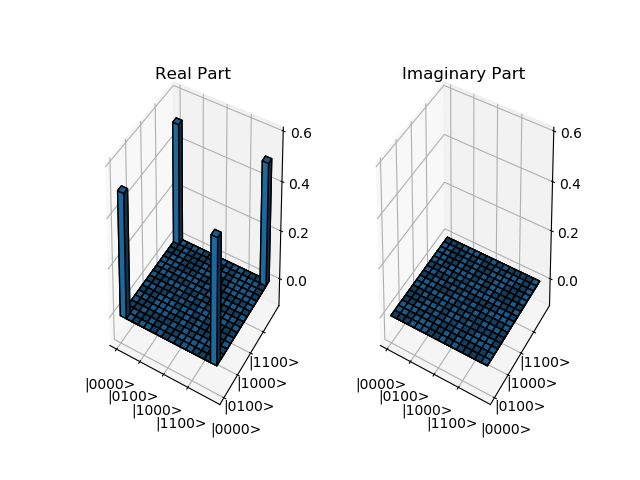
\includegraphics[clip,width=12.0cm]{./picture/1111ed.png}
			\caption{Case 1}
	\end{figure}
	
	\newpage

	\begin{description}
		\item[Case 2:] 理想状態が$\ket{\psi} = \frac{1}{4} (\ket{0000} + \ket{0001} + \ket{0010} + \ket{0011} + \ket{0100} + \ket{0101} + \ket{0110} + \ket{0111} + \ket{1000} + \ket{1001} + \ket{1010} + \ket{1011} + \ket{1100} + \ket{1101} + \ket{1110} + \ket{1111})$の場合 
	\end{description}
	
	\begin{figure}[htbp]
		\centering
			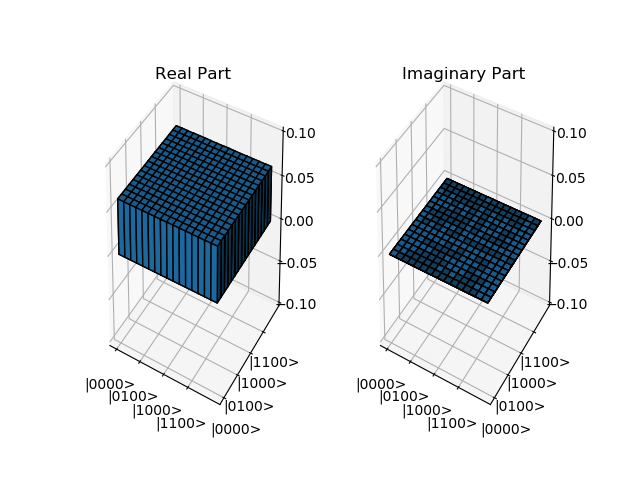
\includegraphics[clip,width=12.0cm]{./picture/all.png}
			\caption{Case 2}
	\end{figure}

	\newpage
	\subsection*{混合状態}

	\begin{description}
		\item[Case 3:] 理想状態が$\hat{\rho} = \frac{1}{6} \{ (\ket{0000} + \ket{1111}) (\bra{0000} + \bra{1111}) + (\ket{0001} + \ket{0010} + \ket{0100} + \ket{1000}) (\bra{0001} + \bra{0010} + \bra{0100} + \bra{1000})\}$の場合 
	\end{description}
	
	\begin{figure}[htbp]
		\centering
			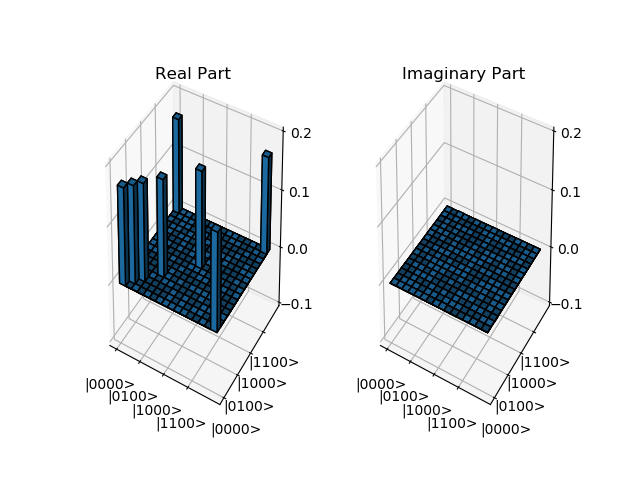
\includegraphics[clip,width=12.0cm]{./picture/mixed.png}
			\caption{Case 3}
	\end{figure}

	\newpage

	\subsection*{計算量・計算時間}

	上記3パターンの計算量は次のとおりである。
	また、最尤推定の初期値を最大混合状態$\hat{I}$にした場合と比較している。

	\begin{figure}[htbp]
		\centering
			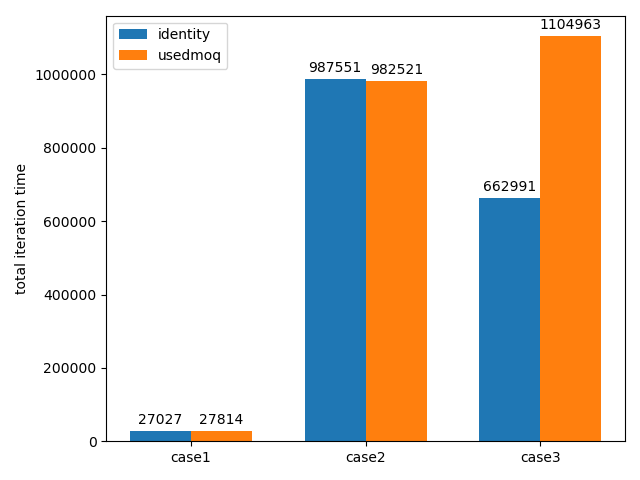
\includegraphics[clip,width=12.0cm]{./picture/cg.png}
			\caption{最尤推定の計算量}
	\end{figure}

	データセットによって計算時間、計算量に大きな違いがあった。
	また、Case 3においては計算量に大きな差が現れた。
	原因として、初期値を予想した場合、初期の更新で尤度関数が減少、つまり密度行列の更新に失敗したために$\epsilon$を小さくして更新が続けられたためである。
	したがって、初期の優位性を保ったまま密度行列を更新することができれば計算量を減らすことができるかもしれないが、そのためには更新ごとに適切な$\epsilon$を見つける必要がある。
	その計算が負担となり総計算時間が減少するとは限らない。

	\newpage

	\subsection*{並列化}

	100個の同じデータセットに対して並列化処理を加えたことで、高速化されました。

	\begin{figure}[htbp]
		\centering
			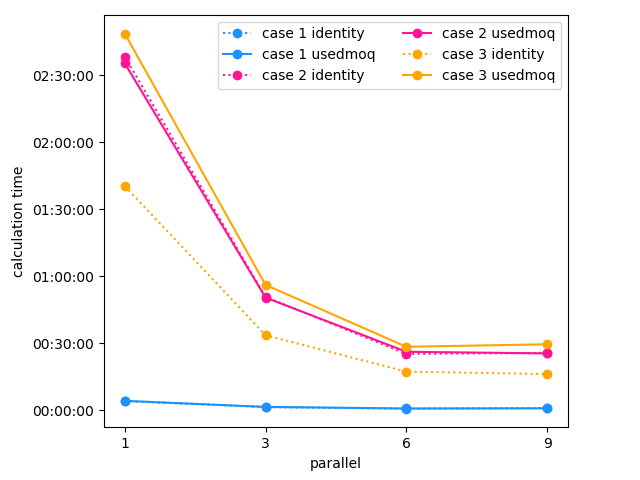
\includegraphics[clip,width=12.0cm]{./picture/parallel.png}
			\caption{並列化した場合の計算時間}
	\end{figure}

	\newpage

	\subsection*{fidelityの推移}

	fidelityとは次の式で求まる二つの量子状態の近さを表す量である。

	\begin{equation}
		F \equiv Tr \sqrt{\sqrt{\hat{\sigma}} \hat{\rho} \sqrt{\hat{\sigma}}}
	\end{equation}

	\begin{figure}[htbp]
		\centering
			\begin{tabular}{c}
	  
			% 1
				\begin{minipage}{0.5\hsize}
				\begin{center}
					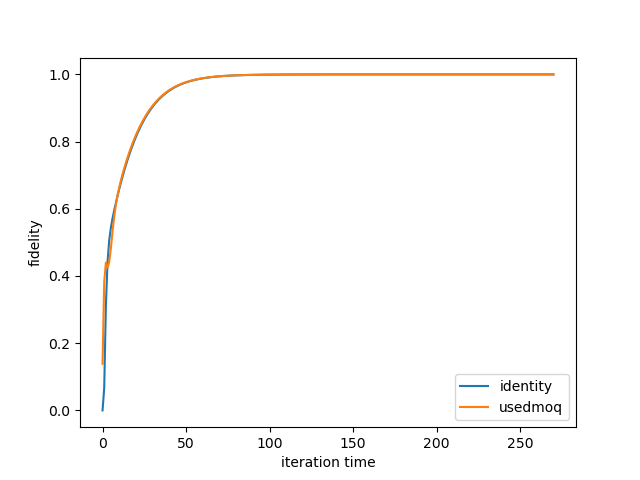
\includegraphics[clip, width=8cm]{./picture/fp1111ed.png}
				\end{center}
				\end{minipage}
	  
			% 2
				\begin{minipage}{0.5\hsize}
				\begin{center}
					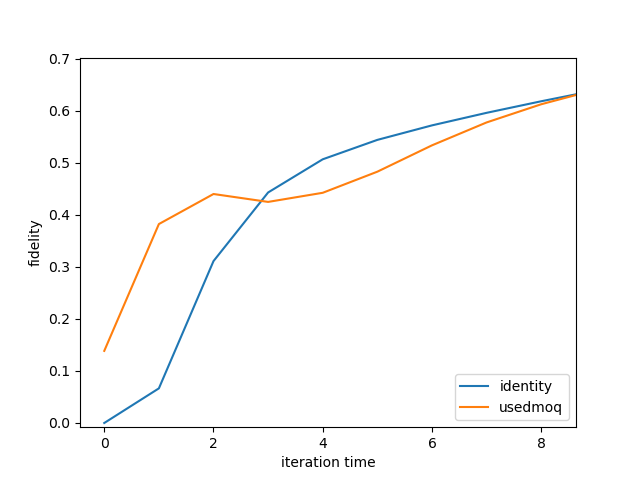
\includegraphics[clip, width=8cm]{./picture/fp1111edextended.png}
				\end{center}
				\end{minipage}
			
			\end{tabular}
		\caption{Case 1}
	\end{figure}

	\begin{figure}[htbp]
	\centering
		\begin{tabular}{c}
	  
			% 1
			\begin{minipage}{0.5\hsize}
			\begin{center}
				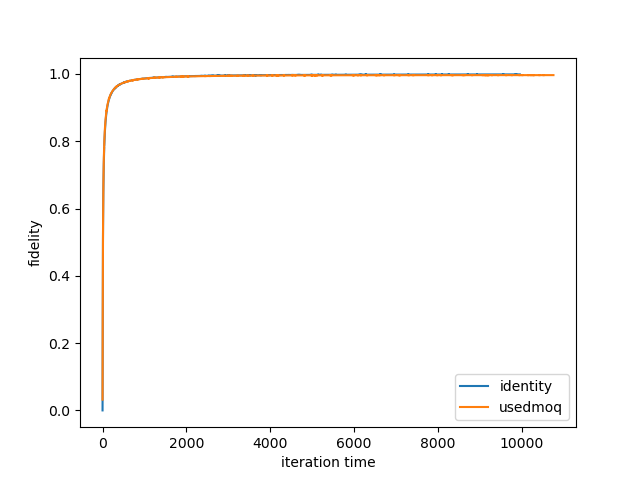
\includegraphics[clip, width=8cm]{./picture/fpall.png}
			\end{center}
			\end{minipage}
	  
			% 2
			\begin{minipage}{0.5\hsize}
			\begin{center}
				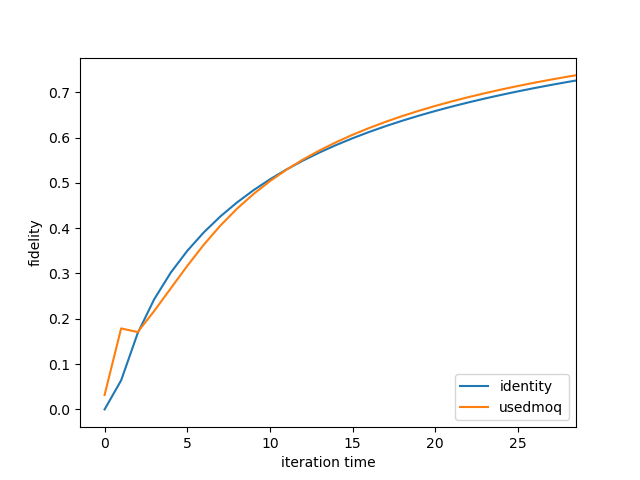
\includegraphics[clip, width=8cm]{./picture/fpallextended.png}
			\end{center}
			\end{minipage}
			
		\end{tabular}
		\caption{Case 2}
	\end{figure}

	\newpage

	\begin{figure}[htbp]
		\centering
			\begin{tabular}{c}
	  
			% 1
			\begin{minipage}{0.5\hsize}
			\begin{center}
				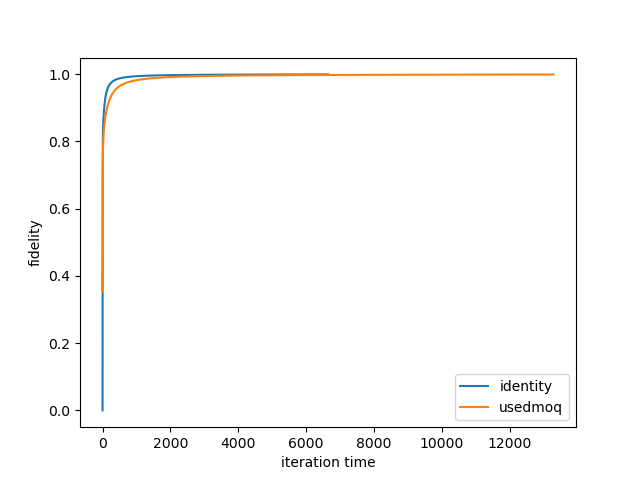
\includegraphics[clip, width=8cm]{./picture/fpmixed.png}
			\end{center}
			\end{minipage}
	  
			% 2
			\begin{minipage}{0.5\hsize}
			\begin{center}
				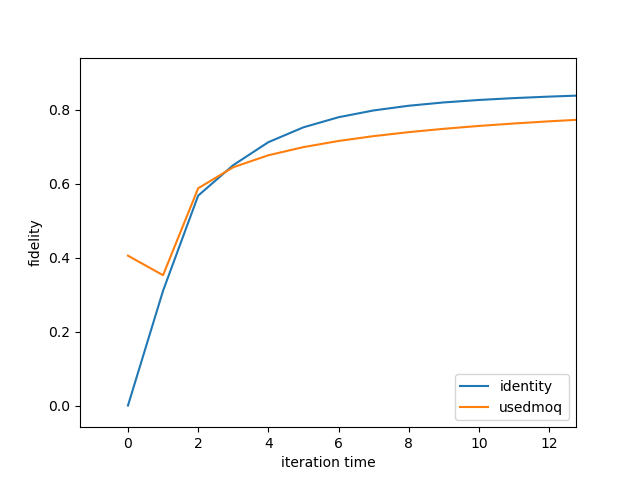
\includegraphics[clip, width=8cm]{./picture/fpmixedextended.png}
			\end{center}
			\end{minipage}
			
		\end{tabular}
		\caption{Case 3}
	\end{figure}

	それぞれのCaseで、初期値を推定した場合の方が初期fidelityは高くなっているが、fidelityの収束値に大きな差はなかった。
	また、いずれの場合にもその後の更新でfidelityの減少が見られた。
	そのために初期の優位性を保ったまま密度行列が更新することができず、総計算量は完全混合状態から始めた場合とあまり変わらなかった。


	\newpage
	\section{quditの結果}

	今回は$d=3$の2 qutritsを実装しました。
	測定基底は~\cite{qutrit}と同じものを使用しました。

	\begin{figure}[htbp]
		\centering
			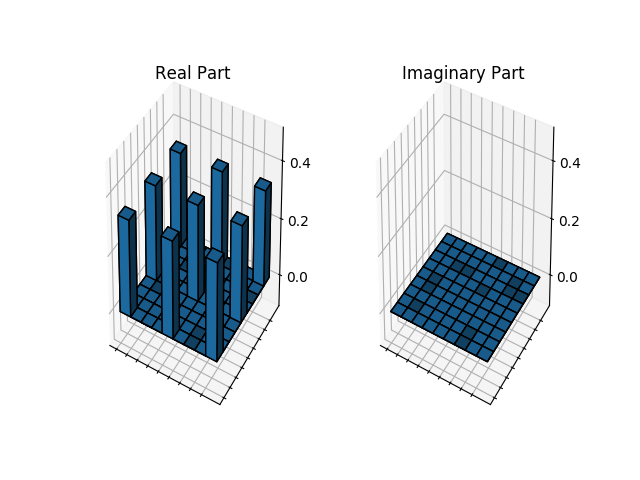
\includegraphics[clip,width=12.0cm]{./picture/qutrit.png}
			\caption{Case 1}
	\end{figure}

	\chapter{まとめ}

	まず初めに1 qubitの量子トモグラフィーを理論的に説明し、その後Multi qubits、1 quditそしてMulti quditsへと拡張していった。
	また、再構成した密度行列が非物理的な値である場合に利用する最尤推定のアルゴリズム($\hat{R} \hat{\rho} \hat{R}$アルゴリズム)を説明し、微小項$\epsilon$を導入することで尤度関数の増加を証明した。

	アルゴリズムの実装では、Multi qubitsでは4 qubitsに対して疑似実験データを生成し、アルゴリズムの有用性を確認した。
	一方、Multi quditsでは$d=3$の2 qutritsに対して同様にシミュレーションで有用性を確認した。
	計算時間の短縮を並列化することで達成した。
	また計算量については、シミュレーション結果から初期値を変えた場合と比較してfidelityの推移からアルゴリズムの改善の必要があることが推察された。


	\chapter*{謝辞}




	\begin{thebibliography}{99}
		\bibitem{}  Michael A. Nielsen, Isaac L. Chuang, Quantum Computation and Quantum Information 10th Aniversary Edition (CAMBRIDGE UNIVERSITY PRESS 2010)
		\bibitem{}  R. T. Thew et al., Qudit quantum-state tomography, Phys. Rev. A 66, 012303 (2002)
		\bibitem{}  Daniel F. V. James et al., Measurement of qubits, Phys. Rev. A 64, 052312 (2001)
		\bibitem{}  J. Rehacek, Z. Hrakil, and M.Jesek, Iterative algorithm for reconstruction of entangled states, Rev. A VOL. 63, 040303 (2001)
		\bibitem{}  Jaroslav Rehacek and Sdenek Hradil et al., Diluted maximum-likelihood algorithm for quantum tomography, Phys. Rev. A 75, 042108 (2007)                                
		\bibitem{}  Z. Hradil, Quantum-state estimation, Phys. Rev. A THIRD VOL. 55, NUMBER 3, R1561 (1996)
		\bibitem{}  Jaromir Fiurasek, Maximum-likelihood estimation of quantum measurement, Phys. Rev. A 64, 024102 (2001)
		\bibitem{qutrit}  Michael Kues et al., On-chip generation of high-dimensional entangled quantum states and their coherent control, Nature 546, pages622–626 (2017) 
	\end{thebibliography}
	


	\appendix

	\chapter{Cholesky Decomposition}
	\label{chap:Cholesky}

	直接計算する。\\

	まず、対角項は
	\begin{equation*}
		\begin{gathered}
			\hat{\rho}_{11} = \big| \hat{T}_{11} \big|^2 + \big| \hat{T}_{21} \big|^2 + \cdots + \big| \hat{T}_{d1} \big|^2 \\
			\hat{\rho}_{22} = \big| \hat{T}_{22} \big|^2 + \big| \hat{T}_{32} \big|^2 + \cdots + \big| \hat{T}_{d2} \big|^2 \\
			\vdots \\
			\hat{\rho}_{ii} = \big| \hat{T}_{ii} \big|^2 + \big| \hat{T}_{i+1\ i} \big|^2 + \cdots + \big| \hat{T}_{di} \big|^2 = \sum_{j=1}^d \big| \hat{T}_{ji} \big|^2 \\
			\vdots \\
			\hat{\rho}_{dd} = \big| \hat{T}_{dd} \big|^2
		\end{gathered}
	\end{equation*}
	非対角項は
	\begin{equation*}
		\begin{gathered}
			\hat{\rho}_{12} = \hat{T}_{21}^\dagger \hat{T}_{22} + \hat{T}_{31}^\dagger \hat{T}_{32} + \cdots + \hat{T}_{d1}^\dagger \hat{T}_{d2} \\
			\hat{\rho}_{13} = \hat{T}_{31}^\dagger \hat{T}_{33} + \hat{T}_{41}^\dagger \hat{T}_{43} + \cdots + \hat{T}_{d1}^\dagger \hat{T}_{d3} \\
			\vdots \\
			\hat{\rho}_{1i} = \hat{T}_{i1}^\dagger \hat{T}_{ii} + \hat{T}_{i+1\ 1}^\dagger \hat{T}_{i+1\ i} + \cdots + \hat{T}_{d1}^\dagger \hat{T}_{di} = \sum_{j=1}^d \hat{T}_{j1}^\dagger \hat{T}_{ji}\\
			\vdots \\
			\hat{\rho}_{1d} = \hat{T}_{d1}^\dagger \hat{T}_{dd} \\
			\vdots \\
			\hat{\rho}_{23} = \hat{T}_{32}^\dagger \hat{T}_{33} + \hat{T}_{42}^\dagger \hat{T}_{43} + \cdots + \hat{T}_{d2}^\dagger \hat{T}_{d3} \\
			\hat{\rho}_{24} = \hat{T}_{42}^\dagger \hat{T}_{44} + \hat{T}_{52}^\dagger \hat{T}_{54} + \cdots + \hat{T}_{d2}^\dagger \hat{T}_{d4} \\
			\vdots \\
			\hat{\rho}_{ij} = \hat{T}_{ji}^\dagger \hat{T}_{jj} + \hat{T}_{j+1\ i}^\dagger \hat{T}_{j+1\ j} + \cdots + \hat{T}_{di}^\dagger \hat{T}_{dj} = \sum_{k=1}^d \hat{T}_{ki}^\dagger \hat{T}_{kj}\ \ \ (i<j)
		\end{gathered}
	\end{equation*}
	より、
	\begin{equation*}
		\begin{gathered}
			\hat{T}_{dd} = \sqrt{\hat{\rho}_{dd}} \\
			\hat{T}_{d\ d-1} = \Big( \frac{\hat{\rho}_{d-1\ d}}{\hat{T}_{dd}} \Big)^\dagger = \frac{\hat{\rho}_{d-1\ d}^\dagger}{\sqrt{\hat{\rho}_{dd}}} \\
			\hat{T}_{d\ d-2} = \Big( \frac{\hat{\rho}_{d-2\ d}}{\hat{T}_{dd}} \Big)^\dagger = \frac{\hat{\rho}_{d-2\ d}^\dagger}{\sqrt{\hat{\rho}_{dd}}} \\
			\vdots \\
			\hat{T}_{d1} = \Big( \frac{\hat{\rho}_{1d}}{\hat{T}_{dd}} \Big)^\dagger = \frac{\hat{\rho}_{1d}^\dagger}{\sqrt{\hat{\rho}_{dd}}} \\
			\hat{T}_{d-1\ d-1} = \sqrt{\hat{\rho}_{d-1\ d-1} - | \hat{T}_{d\ d-1} |^2} = \sqrt{\hat{\rho}_{d-1\ d-1} - \frac{(\hat{\rho}_{d-1\ d}^\dagger)^2}{\hat{\rho}_{dd}}} \\
			\hat{T}_{d-1\ d-2} = \Bigg(\frac{\hat{\rho}_{d-2\ d-1} - \hat{T}_{d\ d-2}^\dagger \hat{T}_{d\ d-1}}{\hat{T}_{d-1\ d-1}} \Bigg)^\dagger = \left( \frac{\hat{\rho}_{d-2\ d-1} - \frac{\hat{\rho}_{d-2\ d}}{\sqrt{\hat{\rho}_{dd}}} \frac{\hat{\rho}_{d-1\ d}^\dagger}{\sqrt{\hat{\rho}_{dd}}}}{\sqrt{\hat{\rho}_{d-1\ d-1} - \frac{(\hat{\rho}_{d-1\ d}^\dagger)^2 }{\hat{\rho}_{dd}}}} \right)^\dagger \\
			\vdots
		\end{gathered}
	\end{equation*}

	このようにして、$\hat{T}_{(t)}$は求まる。
	
		















\end{document}